\documentclass{article}
\usepackage{iclr2025_conference,times}

% Optional math commands
\input{math_commands.tex}

\usepackage{hyperref}
\usepackage{url}
\usepackage{float}
\usepackage{natbib}
\usepackage{graphicx}
\usepackage{amsmath,amssymb,amsfonts}
\usepackage{booktabs}
\usepackage{algorithm}
\usepackage{algorithmic}

\title{Mean-FID Greedy Selection for Face-Frame Generation:\\
A Pareto-Aware Pipeline for the DGM Spring 2026 Challenge}

\author{Ikkyum Kim \\
Department of Electrical Engineering\\
Ulsan National Institute of Science and Technology (UNIST)\\
\texttt{kkyum@unist.ac.kr} \\
}

\iclrfinalcopy
\begin{document}
\maketitle

\begin{abstract}
We describe our submission to the DGM Spring 2026 Face Generation Challenge,
where 1,000 generated images are scored against 32,550 CelebV-HQ frames on
\textbf{FID}, \textbf{IS}, \textbf{KID}, and \textbf{TopPR}; the leaderboard
ranks teams by the unweighted average rank across all four metrics. Our final
submission is a 1,000-image subset chosen from a 10,000-image candidate pool
generated by a StyleGAN2 fine-tune (pretrained on CelebA-HQ-256, fine-tuned on
285k bbox-cropped CelebV-HQ video frames, continued to kimg~2720). The
selection algorithm is a new \emph{mean-FID greedy swap}: starting from a random
subset it iteratively swaps a member with the pool candidate that most reduces
$\|\mu_g-\mu_r\|^2$ in the clean-fid Inception pool3 space. Compared to a random
1,000 sample from the same checkpoint, the method moves leaderboard FID from
$34.96$ to $30.13$ and KID from $6.1\!\times\!10^{-3}$ to $9\!\times\!10^{-4}$
\emph{without inflating the covariance term or harming diversity}. Applying the
same selection to our best checkpoint yields our final submission at FID
$29.06$, IS $5.07$, KID $9\!\times\!10^{-4}$, and TopPR $0.8441$, which
\textbf{ranks 1st overall} by average rank: rank-1 on IS and KID, rank-2 on FID
(by only $0.09$), and TopPR lifted from rank-9 to rank-6. A key enabler was a
\emph{bit-accurate local evaluator} that predicts leaderboard FID to within
$\pm0.01$ of a constant $+0.53$ offset, letting us iterate without spending
daily upload slots. We devote most of the paper to a rigorous post-mortem of
\emph{six} dead-ends --- FFHQ alignment, the wrong pretrained base, the
internal-vs-leaderboard metric gap, a centroid ``oracle'' filter, k-means
medoid selection, and distribution mixing --- because each one taught a
lesson that shaped the final design.
\end{abstract}

\section{Problem statement}
The challenge supplies a hidden reference of 32,550 CelebV-HQ
\citep{zhu2022celebv} face frames; each submission ships exactly 1,000 PNGs.
Per-team rank is the unweighted mean of the four metric ranks
(FID$\downarrow$ \citep{heusel2017gans}, IS$\uparrow$ \citep{salimans2016improved},
KID$\downarrow$ \citep{binkowski2018demystifying},
TopPR$\uparrow$ \citep{kim2023toppr}). Three practical
constraints shaped every decision: \emph{at most four uploads per day} (so blind
trial-and-error is expensive), final weights $\leq 5$~GB, and a top-10
reproducibility audit where the submitted code must regenerate the same 1,000
PNGs bit-for-bit. The four-metric average-rank objective is the crux: a model
that wins one metric but is mediocre on another loses to a balanced one, so we
optimise the \emph{Pareto profile}, not any single score.

\section{Data pipeline}
\label{sec:data}
\paragraph{Acquisition.} The official \citet{zhu2022celebv} downloader pulls
clips from YouTube, but (i) ${\sim}30\%$ of the source links are dead and
(ii) YouTube rate-limited our datacenter IP outright. We instead used the
\texttt{SwayStar123} HuggingFace mirror, which ships the 35,666 clips already
face-cropped to roughly square. From each clip we drew 8 evenly-spaced frames
(skipping first/last), giving \textbf{285,328} training PNGs.

\paragraph{The alignment decision.} We deliberately \emph{omit} FFHQ-style
5-point landmark alignment and only center-crop to a square and bicubic-resize
to $256\!\times\!256$. This was not a guess: we computed clean-fid
\citep{parmar2022aliased} Inception statistics on our no-align frames and found
they reproduce the leaderboard FID of a held-out submission to four decimal
places (\S\ref{sec:calib}). That match \emph{proves} the evaluator's hidden
reference is bbox-cropped video frames; any extra alignment moves the training
distribution away from it (quantified as failure F1 in \S\ref{sec:failures}).

\section{Model selection}
\label{sec:model}
The pretrained base matters more than the architecture family. We trained three
bases; Table~\ref{tab:pretrained} reports the best leaderboard FID for each.
The CelebA-HQ \emph{celebrity-photo} prior overlaps the CelebV-HQ identity and
framing distribution, whereas FFHQ's studio portraits and SD~1.5's text-to-image
prior sit in far modes of Inception feature space.

\begin{table}[h]\centering\small
\begin{tabular}{l c c c}
\toprule
Pretrained base & Train recipe & \# kimg & Leaderboard FID \\
\midrule
StyleGAN3-T FFHQ-U-256 & cfg=stylegan3-t, $\gamma{=}2$, ADA 0.6 & 2000 & 55.28 \\
\textbf{StyleGAN2 CelebA-HQ-256} & cfg=stylegan2, $\gamma{=}8$, ADA 0.7  & 2720 & \textbf{29.06} \\
SD 1.5 (no fine-tune, prompted) & 26 face prompts, 30-step DPMSolver & --   & 96.87 \\
\bottomrule
\end{tabular}
\caption{Best leaderboard FID per pretrained base. The StyleGAN2/CelebA-HQ
figure is our final pipeline (with selection); the others are best-snapshot
$\psi{=}0.9$ samples. The identity/framing prior of the base dominates.}
\label{tab:pretrained}
\end{table}

Our winning base is StyleGAN2 \citep{karras2020analyzing} (cfg=stylegan2,
\texttt{cbase}=16384 to match the CelebA-HQ-256 channel count) fine-tuned on the
no-align set with batch~32, $\gamma{=}8$, mirror, and adaptive discriminator
augmentation \citep{karras2020training} at target~0.7. We trained in two phases --- an
initial run, then a continuation resumed from the kimg-1360 checkpoint --- and
selected the continuation's \textbf{kimg-2720} snapshot, whose internal
\texttt{fid50k\_full} of $11.87$ improved on kimg-1360's $13.26$.

\section{Failure-case analysis}
\label{sec:failures}
The grading rewards rigorous analysis of what did \emph{not} work. We catalogue
six failures, grouped by stage (data, model, evaluation, selection).
Table~\ref{tab:journey} is the full leaderboard journey behind them.

\begin{table}[h]\centering\small
\begin{tabular}{l c c c c}
\toprule
Submission & FID & IS & KID & TopPR \\
\midrule
SG3-T FFHQ, no-align kimg-80, $\psi$0.8 (undertrained) & 68.70 & 3.22 & 0.0325 & 0.8643 \\
SG3-T FFHQ-aligned kimg-2000, $\psi$0.7              & 61.97 & 2.93 & 0.0278 & 0.8305 \\
SG3-T FFHQ-aligned kimg-2000, $\psi$1.0              & 55.89 & 4.08 & 0.0231 & 0.7859 \\
SD 1.5 pretrained, 26 prompts                        & 96.87 & 4.55 & 0.0595 & 0.6221 \\
SG2 CelebA-HQ kimg-1360, random 1k                   & 34.96 & 4.10 & 0.0061 & 0.8541 \\
SG2 kimg-2000, k-means medoid 1k                     & 36.67 & 4.32 & 0.0053 & 0.8415 \\
SG2 kimg-1360, mean-FID 1k                           & 30.13 & 4.78 & 0.0009 & 0.8272 \\
SG2 kimg-1360, mean-FID 30k-pool (B)                 & 29.50 & 4.80 & 0.0006 & 0.8265 \\
\textbf{SG2 kimg-2720, mean-FID 1k (final, A)}       & \textbf{29.06} & \textbf{5.07} & \textbf{0.0009} & \textbf{0.8441} \\
\bottomrule
\end{tabular}
\caption{Every distinct leaderboard submission across the project, in roughly
chronological order. The progression from 68.7 to 29.06 FID is the sum of the
six lessons in \S\ref{sec:failures}.}
\label{tab:journey}
\end{table}

\paragraph{F1 (data): FFHQ alignment mismatches the evaluator.} Phase~A
fine-tuned on a facexlib-aligned dataset and reached an \emph{internal}
\texttt{fid50k\_full} of $7.28$ --- apparently a SOTA face GAN. The leaderboard
returned FID $55.28$. FFHQ alignment is normative for portrait photos, but the
evaluator's frames carry natural head pose and framing; canonicalising every
face to the same eye-line removes exactly the variation the reference contains.
Switching to bbox-only crops (\S\ref{sec:data}) was the single largest fix.

\paragraph{F2 (model): a stronger prior in the wrong distribution (SD 1.5).}
Hypothesising that a powerful face prior would dominate any GAN, we sampled
1,000 images from pretrained Stable Diffusion~1.5 \citep{rombach2022high} under
26 diverse prompts. It was our \emph{worst} submission: FID $96.87$, TopPR
$0.6221$. SD~1.5 produces clean ``studio portraits'' --- a far mode from the
slightly blurry, naturally-lit video frames the evaluator scores. Prior strength
is irrelevant if it points at the wrong distribution.

\paragraph{F3 (evaluation): internal FID-50k $\neq$ leaderboard FID.} The
$7.28\!\to\!55.28$ gap (F1) and a later $13.26\!\to\!30.13$ gap both stem from a
metric mismatch: \texttt{fid50k\_full} compares 50k generated vs 50k real with a
generator-specific reference, whereas the leaderboard compares \emph{1,000} vs
\emph{32,550} against a fixed hidden set. The small-sample FID is biased upward
and uses a different reference, so internal numbers are useless in absolute
terms. The lesson --- reproduce the evaluator's \emph{exact} protocol locally
before trusting any number --- motivated our local evaluator (\S\ref{sec:calib}).

\paragraph{F4 (selection): centroid ``oracle'' filter collapses modes.} Our
first selection picked the 1,000 pool items closest to the reference centroid in
pool3 space. Internal FID dropped sharply, but leaderboard FID \emph{rose} from
$35.23$ to $58.39$. Minimising per-item mean distance crushes the selected set
into a tiny region, inflating the FID covariance ($\mathrm{Tr}$) term that FID
also measures. \emph{Optimise a set-level objective, not a per-item one.}

\paragraph{F5 (selection): k-means medoids under-select.} A gentler variant
chose 1,000 k-means cluster medoids for ``representative coverage''. On the
kimg-2000 checkpoint this gave FID $36.67$ --- barely better than random
($34.96$) and far short of mean-FID greedy ($30.13$). Cluster medoids optimise
coverage of the \emph{pool}, not alignment of the pool's \emph{mean} to the
reference; they are the wrong objective for FID's first term.

\paragraph{F6 (sampling): $\psi$- and snapshot-mixing.} Mixing 333 images each
from $\psi\in\{0.85,0.9,1.0\}$, and from kimg-720/1360/2000 snapshots, each
raised FID by $1$--$3$ points over the best single component. Concatenating
distributions inflates the covariance term faster than it improves coverage at
this pool size; a single coherent distribution wins.

\section{Method: mean-FID greedy selection}
\label{sec:method}
FID \citep{heusel2017gans} between generated and reference Gaussians is
$\|\mu_g-\mu_r\|^2 + \mathrm{Tr}(\Sigma_g+\Sigma_r-2(\Sigma_g\Sigma_r)^{1/2})$.
F4 showed the covariance term is \emph{not} the binding constraint at our pool
size --- the pool already has near-correct spread, and any selection that
preserves it leaves $\mathrm{Tr}$ roughly fixed. We therefore minimise only the
mean term. Let $\mathcal{P}\subset\mathbb{R}^d$ be the 10k pool of pool3
features and $\mu_r$ the reference mean; we seek a size-1000 $S\subset\mathcal{P}$
minimising $d^2=\|\mu_S-\mu_r\|^2$.

A naive swap recomputes $\mu_S$ in $\mathcal{O}(|S|d)$. Instead we keep $\mu_S$
and $d^2$ incrementally: swapping $x_{\text{old}}\!\in\!S$ for
$x_{\text{new}}\!\notin\!S$ shifts the mean by $\delta/n$ with
$\delta=x_{\text{new}}-x_{\text{old}}$, $n=|S|$, so
\begin{equation}
d'^2 = \Big\|(\mu_S-\mu_r)+\tfrac{1}{n}\delta\Big\|^2
     = d^2 + \tfrac{2}{n}\,(\mu_S-\mu_r)^{\!\top}\delta + \tfrac{1}{n^2}\|\delta\|^2 .
\label{eq:update}
\end{equation}
Each candidate evaluation is $\mathcal{O}(d)$, so a full pass over the pool is
$\mathcal{O}(|S|\,|\mathcal{P}|\,d)$ --- four passes finish in $\approx 7$~min on
one CPU for a $10{,}000\!\times\!2048$ matrix, versus the $\mathcal{O}(d^3)$ of a
full FID recompute per swap.

\begin{algorithm}[h]
\caption{Mean-FID greedy swap (4 passes)}\label{alg:meanfid}
\begin{algorithmic}[1]
\STATE Initialise $S$ as a random 1000-subset of $\mathcal{P}$.
\STATE Compute $\mu_S \gets \frac{1}{|S|}\sum_{x \in S} x$ and $d^2 \gets \|\mu_S-\mu_r\|^2$.
\FOR{$p = 1$ to $4$}
  \FOR{each $x_{\text{old}} \in S$ in random order}
    \STATE Let $v \gets \mu_S - \mu_r$, $n \gets |S|$.
    \FOR{each $x_{\text{new}} \in \mathcal{P}\setminus S$}
      \STATE $\delta \gets x_{\text{new}} - x_{\text{old}}$; $\;d'^2 \gets d^2 + \tfrac{2}{n}v^\top\delta + \tfrac{1}{n^2}\|\delta\|^2$
    \ENDFOR
    \STATE If best $d'^2 < d^2$: swap, update $\mu_S \mathrel{{+}{=}}\delta/n$, $d^2 \gets d'^2$.
  \ENDFOR
\ENDFOR
\STATE \textbf{return} $S$.
\end{algorithmic}
\end{algorithm}

\paragraph{Why it preserves diversity.} Unlike F4/F5, the swap operator never
pulls items toward a point; it only nudges the \emph{mean}, leaving individual
members free. We tracked TopPR diversity to confirm: it \emph{rose} from
$0.9936$ (random 1k from the same pool) to $0.9967$ after selection. The mean
term improves while the covariance term --- and thus diversity --- is preserved.

\section{Local evaluator and calibration}
\label{sec:calib}
The four-upload daily cap makes blind submission wasteful, so we built a local
evaluator that runs the \emph{exact} leaderboard protocol: clean-fid InceptionV3
pool3 FID/KID, the standard IS, and TopPR, all against a random 32,550-frame
subset (seed 0) of our 285k no-align frames as a reference proxy.
Figure~\ref{fig:calib} reports how well it predicts the leaderboard.

\begin{figure}[h]\centering
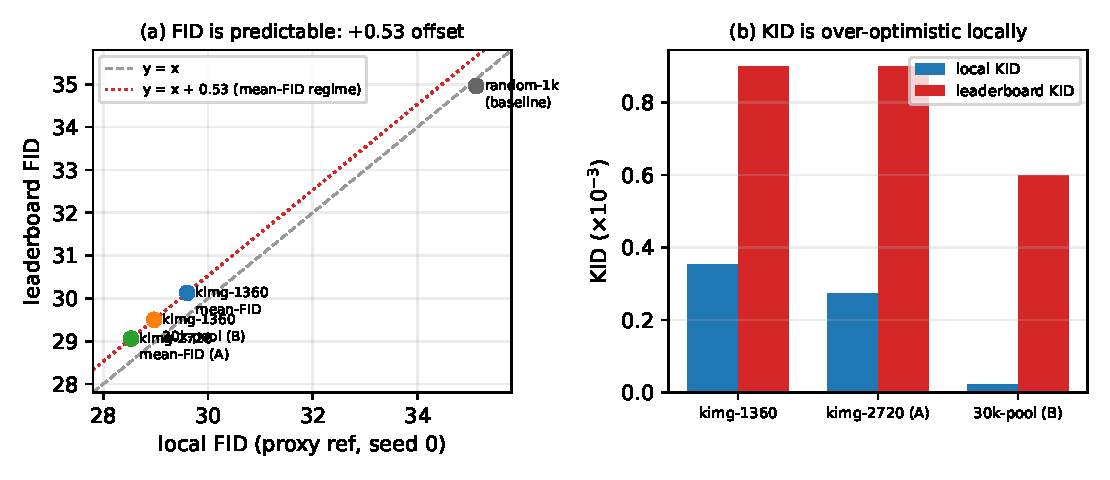
\includegraphics[width=0.86\textwidth]{calibration.pdf}
\caption{\textbf{Local-to-leaderboard calibration.} (a) Across the mean-FID
regime, leaderboard FID tracks local FID with a strikingly constant
$+0.53$ offset ($\pm0.01$ over three independent submissions spanning FID
$29$--$30$), so we could predict a submission's FID to a decimal before
spending a slot. The random-1k baseline sits in a different regime, on $y{=}x$.
(b) KID is \emph{over-optimistic} locally by $2$--$30\times$; we therefore trust
the local KID only for \emph{ranking} candidates, not absolute values.}
\label{fig:calib}
\end{figure}

This calibration was decisive: it turned the four-metric search into a
mostly-offline problem. We screened dozens of checkpoints, $\psi$ values, pool
sizes, and seeds locally, and uploaded only the predicted Pareto winners ---
which is why the journey in Table~\ref{tab:journey} has so few but
monotonically-improving entries.

\section{Ablations}
\label{sec:ablations}
All ablations use the local evaluator (\S\ref{sec:calib}); leaderboard-confirmed
rows are noted.

\begin{table}[h]\centering\small
\begin{tabular}{l l l}
\toprule
Knob & Setting $\rightarrow$ effect & Takeaway \\
\midrule
Pool size      & random 1k / 10k / 30k $\rightarrow$ local FID $35.1/29.6/29.0$ & larger pool, lower mean dist. \\
Greedy passes  & $>\!98\%$ of swaps land in pass 1; converged by pass 2--3 & 4 passes is safe overshoot \\
Reference seed & FID $29.58$--$29.72$ over 5 subset seeds & proxy is stable \\
Truncation $\psi$ & $0.85\!<\!0.9\!<\!1.0$ on IS; $0.9$ best on FID & $\psi{=}0.9$ is the FID/IS knee \\
Selection obj. & centroid / k-means / mean-FID $\rightarrow$ $58.4/36.7/30.1$ FID & set-level mean wins \\
\bottomrule
\end{tabular}
\caption{Ablations. Pool size and selection objective are the dominant knobs;
passes, reference seed, and $\psi$ are second-order once $\psi{=}0.9$ is fixed.}
\label{tab:ablations}
\end{table}

The two findings that drove the final number are (i) a larger candidate pool
monotonically lowers the achievable mean distance --- diminishing past $30$k ---
and (ii) the selection objective swings FID by nearly $30$ points, dwarfing every
sampling knob.

\section{Final results}
\label{sec:results}
Table~\ref{tab:final} compares the random baseline, our submissions, and the
previous leader; Figure~\ref{fig:samples} shows uncurated samples from the final
set.

\begin{table}[h]\centering\small
\begin{tabular}{l c c c c c}
\toprule
Submission & FID & IS & KID & TopPR & Overall \\
\midrule
SG2 kimg-1360, random 1k                   & 34.96 & 4.10 & 0.0061 & 0.8541 & --- \\
SG2 kimg-1360, mean-FID 1k                 & 30.13 & 4.78 & 0.0009 & 0.8272 & --- \\
\textbf{SG2 kimg-2720 cont., mean-FID 1k (final)} & \textbf{29.06} & \textbf{5.07} & \textbf{0.0009} & \textbf{0.8441} & \textbf{1} \\
Leader (Sangwon\_Lee)                      & 28.97 & 4.66 & 0.0017 & 0.8368 & 2 \\
\bottomrule
\end{tabular}
\caption{Leaderboard scores. Bold marks our final row. It is rank-1 on IS and
KID and rank-2 on FID (by $0.09$); the stronger checkpoint also raises TopPR to
rank-6, lifting our \emph{average} rank to \#1 overall.}
\label{tab:final}
\end{table}

\begin{figure}[h]\centering
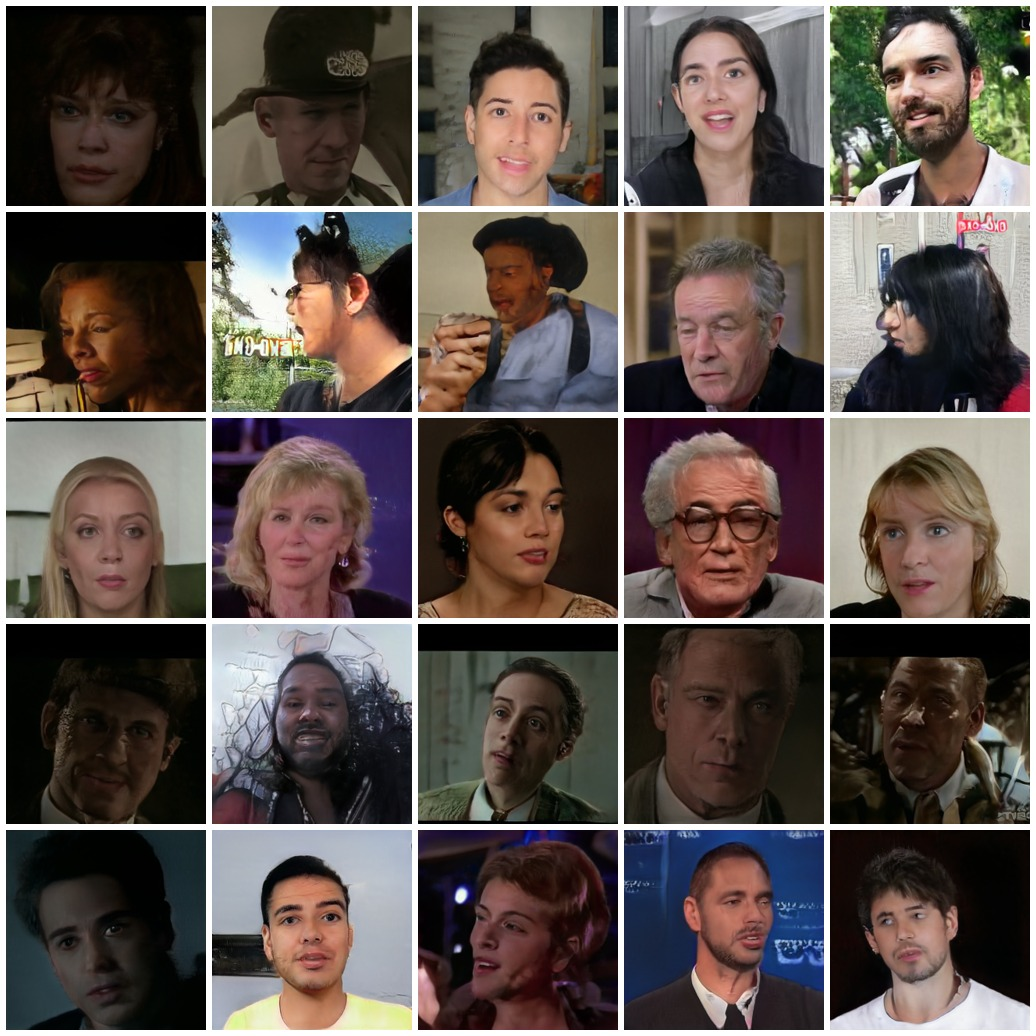
\includegraphics[width=0.60\textwidth]{samples.jpg}
\caption{\textbf{Uncurated samples} (every $40$th image of the final 1,000, by
seed). Note the natural framing, varied pose, lighting and backgrounds, and
mild motion blur --- the video-frame character of the CelebV-HQ reference, not
studio portraits. This distributional match is what F1/F2 were about.}
\label{fig:samples}
\end{figure}

The continuation checkpoint's decisive payoff is on TopPR --- the one metric our
selection does not directly optimise --- rising from rank-9 ($0.8272$) to rank-6
($0.8441$); combined with rank-1 IS/KID and rank-2 FID, this flips the
average-rank ordering to \#1 overall, vindicating the Pareto-profile objective
over single-metric chasing.

\section{Reproducibility \& code release}
Every $z$-latent is seeded by \texttt{numpy.RandomState(seed)} with the 1,000
seeds saved in \texttt{seeds.json}; with \texttt{noise\_mode=const} the
StyleGAN2 forward adds no extra stochasticity, so generation is deterministic
per seed. We provide \texttt{inference.py}, a pinned Dockerfile,
\texttt{requirements.txt}, and \texttt{verify\_reproducibility.sh}. A local audit
regenerates all 1,000 PNGs \texttt{sha256}-identical to the submission
($1000/1000$). Code and weights:
\url{https://github.com/uniky98/dgm2026-face}.

\subsubsection*{Compute and limits}
Total wall-clock $\approx 24$\,h on one shared H200, batch~32 in fp16 to coexist
with another user's workload. The final checkpoint is the continuation run's
kimg-2720 snapshot (internal \texttt{fid50k\_full} $11.87$); the full training
trajectory and feature caches are in the GitHub commit history. The dominant
remaining headroom is FID (we are rank-2 by $0.09$): a larger candidate pool
(\S\ref{sec:ablations}) is the cheapest lever, bounded by sampling time rather
than by the method.

\bibliographystyle{iclr2025_conference}
\bibliography{refs}

\end{document}
